%-------------------------------------------------------------------------------
\section{Introduction}
%-------------------------------------------------------------------------------
Web application developers today have more incentives than ever to provide better privacy for their
users.
%
Laws like the EU's General Data Protection Regulation (GDPR)~\cite{eu:gdpr} and California's
Consumer Privacy Act (CCPA)~\cite{ca:privacy-act} codify users' right to be forgotten, and restrict
any data retention to anonymized information.
%
Legal consequences and the reputational damage associated with data breaches~\cite{breach:amazon,
breach:twitter, breach:fb, breach:marriott, breach:quora} make it good practice to minimize the user
data retained.
%

%
Although many developers are well-intentioned, today they must manually implement \emph{privacy
transformations}---such as user account deletion or data minimization---which burdens
them with complexity and results in ad-hoc solutions. %(\S\ref{sec:survey}).
%\lyt{add other examples of transformations? e.g., anonymization when exporting data, for data
%minimization, to support user-chosen privacy settings? we do only really talk about user account
%deletion in webapps today, though}
%
%
To write a privacy transformation, developers must carefully map the high-level privacy policy to
operations that delete or rewrite data objects, while ensuring that the application preserves
utility for other users, retains legally-mandated anonymized data, and avoids violating application
invariants.
%
For example, deleting a user's account should not unexpectedly grant broad access to
previously-private content by deleting objects that restrict access, nor should it make
non-sensitive shared content disappear.
%
Developers must also consider indirectly identifying correlations between data objects: for example,
anonymized public running routes can identify the user's hometown and even the
user~\cite{strava:heatmap}, and anonymized order histories in e-commerce sites can reidentify
buyers.

\begin{figure}[t]
    \centering
    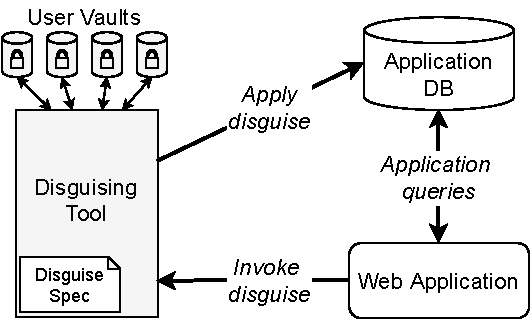
\includegraphics[width=0.35\textwidth]{img/disguise_tool}

    \caption{A data disguising tool sits alongside the application code and database.}
    \label{fig:tool}
\end{figure}


\iffalse
To get privacy transformations right, developers must carefully map the high-level privacy
policy to operations that delete or rewrite data objects, while ensuring that the application preserves
utility for other users, retains legally-mandated anonymized data, and avoids violating
application invariants.
%
For example, deleting a user's account should not unexpectedly grant broad
access to previously-private content by deleting objects that restrict access,
nor should it make non-sensitive shared content disappear.
%
Privacy transformation designers must correctly handle identifying data, as well as indirectly identifying
correlations between data objects.
For example, anonymized public running routes can identify the user's hometown and be
reassociated with the user~\cite{strava:heatmap},
%anonymized posts on Reddit correlated with a subreddit with very few subscribers can be
%associated back to a single user;
% papers' affiliation and reviewer conflicts in HotCRP can reidentify the author;
and anonymized order histories in e-commerce sites can reidentify buyers.
\fi

%
The burden of implementing privacy transformations grows with the underlying privacy policy's
complexity.
%
Although simplicity has advantages, more nuanced privacy policies are important and useful.
%
Such policies can help protect users against data correlation attacks; they can give more
control to individuals by allowing them to choose their own, fine-grained privacy semantics; and
they may enable new privacy modes such as data that gradually ``decays'' to become less identifiable over time.
%
Likewise, reversible privacy transformations might strike a sweet
spot---allowing users to remove identifiable information on demand,
but accommodating service providers' interest to make it easy for users to return---but
add significant implementation burden.
%

%
With more nuanced and reversible privacy transformations, developers face an even greater challenge:
they must reason about how these privacy transformations compose. For example, an application may
automatically decay data over time, but must still correctly remove a user's data when they delete
their account, even if this data has been anonymized.
Ensuring that one privacy transformation does not affect the privacy properties
achieved by future transformations, even if they both transform the same data, is a non-trivial task.
%

%
We propose \emph{data disguising}, a new framework
for systematically specifying, implementing, and reasoning about  privacy transformations.
%
In this framework, developers specify transformations required in privacy policies as
high-level \emph{data disguises} over existing application data types and associations.
%
Applying a disguise transforms the state of application data in privacy-preserving ways (\eg
deleting users' identifiers, or decorrelating identifying object relationships) while preserving
application invariants and utility.
%
Disguises do not guarantee strict privacy---a disguise's content might still expose user
information or correlated data if not redacted by the policy---but flexible disguising,
rather than universal deletion, is what real applications require.
%
%Disguises consist of transformations performed on the high-level object graph embedded in
%database-based applications (encoded by \eg foreign key relationships in relational
%databases)~\cite{orms}.

A data disguising tool takes a disguise and its target, and automatically applies the appropriate
transformations to application data to achieve the disguised state, handling
disguise composition and disguise interdependencies. Developers can
thus reason at a high level about each disguise in isolation, reducing the developer burden.
%

Our proof-of-concept, \sys, demonstrates the potential of such a tool.
%
\sys proxies relational database operations and exposes APIs to invoke privacy transformations.
%
